
Two-Level Segregated Fit (TLSF) is a dynamic storage allocator by M. Masmano et al.~\cite{TLSF}. It is especially designed to be used in real-time applications, where it stands out among other allocators in that it has a bounded and short response time and maintains low fragmentation, thus ensuring high predictability. 

\subsection{Allocation and Freeing Strategy}

From the perspective of the user, TLSF has the same interface as \texttt{malloc()} and \texttt{free()} in libc~\cite{mallocman}. What makes TLSF unique is its internal mechanisms, which are discussed next.

When the user requests N bytes from the allocator, the allocator aligns N to meet any necessary alignment requirements and applies padding. Subsequently, it checks the free-list matching the allocation request to see if it contains any block(s). If no block is found in the list, the allocator checks if any free-list contain blocks larger than the requested size. If no list containing large enough blocks is found, NULL is returned. However, if a list containing block(s) of large enough size is found, the allocator removes the first block in the list, regardless of the number of blocks in it. The policy of searching for free-lists and choosing the first block is called Good-Fit by the authors, referred to as a combination of best- and first-fit. Good-Fit performs well in that search times are low and block sizes often align with the allocation request, requiring little to no additional overhead. Moreover, if a block larger than the requested size is located, the allocator splits it into two blocks. One block is used to satisfy the request to the user, and the other is inserted back into the allocator. Figure~\ref{fig:tlsf_allocation} shows this process.

\begin{figure}[H]
    \centering
    \includesvg[width=1.0\textwidth]{figures/tlsf_allocation.svg}
    \caption{The process of allocating memory in the TLSF allocator.}
    \label{fig:tlsf_allocation}
\end{figure}

When a block is freed, TLSF tries to coalesce the block with its neighboring blocks if they are free. Immediately coalescing when freeing allows the allocator to have larger blocks available for larger request sizes as often as possible. Having as few small blocks as possible minimizes fragmentation. After coalescing has been attempted, the block is inserted into the free-list matching its final size.

\subsection{Technical Description}

The name Two-Level Segregated Fit reflects its design as a free-list based allocator that uses segregated-fit, storing multiple free-lists containing blocks of set size classes. To efficiently lookup what free-list are non-empty, TLSF employs two levels of bitmaps. A first-level bitmap for size classes that are separated by powers of two and a second-level bitmap that subdivides the first-level size classes linearly. In the reference implementation, the number of first- and second-levels are both limited to 32 in order to fit in 32 bits. Additionally, the number of second-levels is recommended to be a power of two for efficiency reasons, so that simple bit-shift instructions can be used. The combined use of multiple free-lists and bitmaps for information bookkeeping enables the asymptotic worst-case response times for allocating and freeing memory to be constant, i.e. \texttt{O(1)}, since it limits the number of instructions for finding blocks.

Allocations inside TLSF are managed using blocks. Blocks are kept track of in two doubly-linked list structures. Initially, blocks are arranged in a physically ordered list by their place in memory, and if a block becomes free, it is then inserted into an appropriate free-list, that is ordered by block size instead. Each block is accompanied by an associated header located next to it. The header specifies the size of the block and also its position within both doubly-linked lists and contains different data depending on if it is free or not. Free blocks contain additional data over allocated blocks, as shown in Figure~\ref{fig:blockheader_reference}.

Moreover, block sizes are aligned to multiples of the allocation unit (4 bytes for a 32-bit architecture). The two least significant bits within the block header are reserved for metadata. These bits indicate whether the block is free (F-bit) and whether it represents the last block within its pool (L-bit), as depicted in Figure~\ref{fig:blockheader_reference}. The F-bit is mainly used to see whether a block can be coalesced and the L-bit to easily iterate over physical blocks.

\begin{figure}[H]
    \centering
    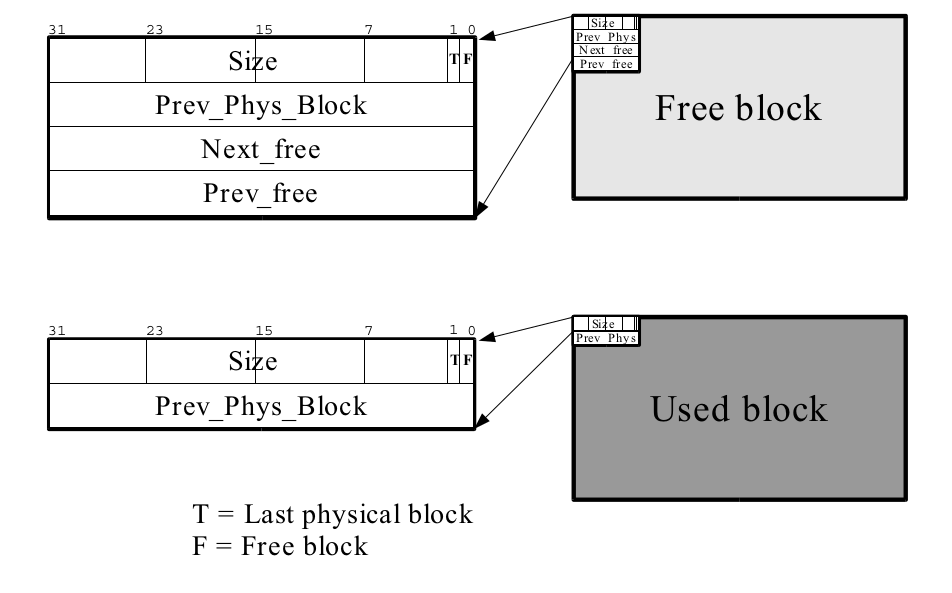
\includegraphics[width=0.60\textwidth]{figures/blockheader_reference.png}
    \caption{Representation of free and allocated block headers in 32-bit architecture. For a 64-bit architecture, each individual field is 8 bytes instead of 4 bytes. (Taken from~\cite{TLSF}).}
    \label{fig:blockheader_reference}
\end{figure}


The TLSF authors primarily focus on low-level allocation primitives, without explicit consideration for garbage collection. Consequently, exploring the adaptation of TLSF to integrate with a garbage collector represents a direction for advancing its development, which is the main focus of this work.

%%% Local Variables:
%%% mode: latex
%%% TeX-master: "main"
%%% End:
